Descargue el archivo disponible en
\begin{center}
\url{https://goo.gl/K2fZZZ}
\end{center}
este archivo contiene una matriz que en su primera columna tiene el precio diario, durante los \'ultimos 22 d\'ias, de la acci\'on de \texttt{Cencosud S.A.} y en su segunda columna la cantidad de acciones transadas de esta empresa en cada d\'ia.

En un rutero de \matlab llamado \texttt{acciones.m}
\begin{enumerate}
\item Calcule el promedio de transacciones diarias para estos d\'ias.
\item Grafique el precio diario de la acci\'on de \texttt{Cencosud S.A.} versus el d\'ia.
\item Calcule y grafique el polinomio interpolante del precio diario de acci\'on de \texttt{Cencosud S.A.}

\textquestiondown Qu\'e observa? \textquestiondown Es confiable este interpolante para preveer futuros valores de esta acci\'on?

\respuesta{5cm}

\item Usando la funci\'on de \matlab \texttt{spline}, calcule y grafique un spline c\'ubico que interpola el precio diario de la acci\'on de \texttt{Cencosud S.A.}
\end{enumerate}
 
\textbf{Desarrollo:} El programa \texttt{cencosud.m} debe tener instrucciones similares a las siguientes
\begin{lstlisting}
clear all; close all; clc;
load('cencosud.mat');
media=mean(cencosud(:,2));		%10 PUNTOS
plot(cencosud(:,1),'+'); hold on;	
pol=polyfit(1:22,cencosud(:,1)',21);
xvec=1:0.1:22;
plot(xvec,polyval(pol,xvec))		%20 PUNTOS

figure(2)
sp=spline(1:22,cencosud(:,1));
plot(xvec,ppval(sp,xvec),1:22,cencosud(:,1)','+') %20 PUNTOS
\end{lstlisting}

con lo que se tiene que 
\begin{lstlisting}
>> media=mean(cencosud(:,2))

media =

   2.5957e+06
\end{lstlisting}

y se generan gr\'aficas como
\begin{center}
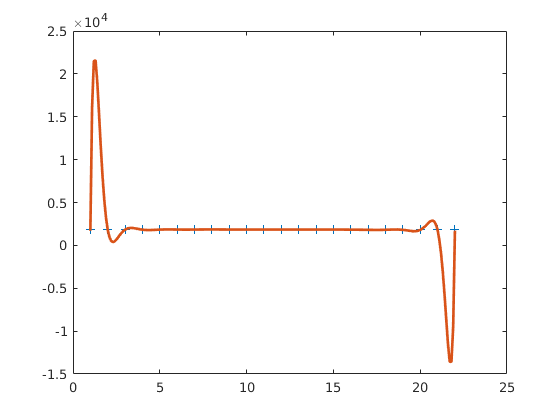
\includegraphics[width=0.8\textwidth]{./cencosud.png}
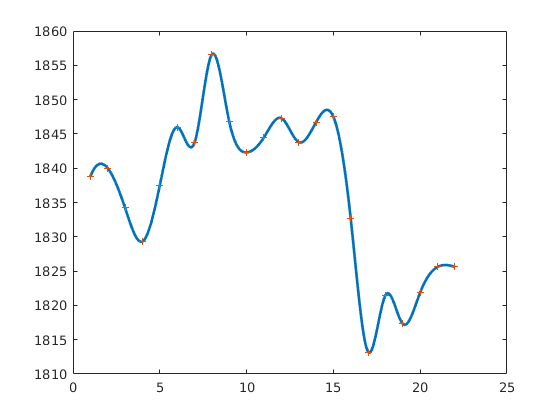
\includegraphics[width=0.8\textwidth]{./cencosud_spline.png}
\end{center}
de donde se responde que, el fen\'omeno de Runge hace poco confiable el interpolante polinomial.

\hfill\fbox{10 puntos}